\chapter{Software Requirements Specification}
\label{chap:software_requirements_specification}

This chapter defines the requirements that guided the design and development of \gls{SafeVision}. It presents the main functional requirements, describes central use cases for detection and redaction, and outlines the non-functional requirements related to security, performance, usability, and maintainability. The chapter also explains how the requirements were prioritized to support a practical development process and ensure that the most important functionality was implemented first.

%------------------------- 4.1 ---------------------------

\section{Functional Requirements}

Functional requirements describe the core capabilities that the system must provide. These requirements are derived from the problem statement and scope in Section~\ref{sec:problem-statement-and-scope}, the project delimitations in Section~\ref{sec:delimitation}, and the stakeholder meetings summarized in Table~\ref{tab:meeting-impact}. The requirements therefore reflect both the original project direction and the practical feedback received from Safe Media AI and the supervisor during development.

\begin{table}[H]
\centering
\begin{tabular}{|p{5cm}|p{9cm}|}
\hline
\textbf{Requirement} & \textbf{Description} \\ \hline

\textbf{Automatic Detection of Sensitive Information} & 
The system shall automatically detect sensitive information in images, including faces and textual content. \\ \hline

\textbf{Image File Support} & 
The system shall support commonly used image formats such as PNG and JPEG. \\ \hline

\textbf{Manual Editing of Detection Results} & 
The system shall allow users to review, modify, and remove detected regions before redaction is applied. \\ \hline

\textbf{Multiple Redaction Methods} & 
The system shall support different redaction techniques such as blurring, pixelation, and \gls{masking}. \\ \hline

\textbf{Redaction Execution} & 
The system shall apply selected redaction methods to user-defined or detected regions. \\ \hline

\textbf{Process Speed} &
The detection process should not be noticeably longer than Safe Media AI's detection system. \\ \hline

\textbf{System Integration Capability} & 
The system should be designed in a way that allows integration with external systems through well-defined interfaces. \\ \hline

\end{tabular}
\caption{Functional Requirements for the \gls{SafeVision} System}
\label{tab:functional_requirements}
\end{table}

%------------------------- 4.2 ---------------------------

\section{Use Case Details}

Use cases further illustrate how users interact with \gls{SafeVision} to achieve the main goals of the system. Whereas the functional requirements define the capabilities the system must provide, the use cases show how these capabilities are combined in practice. For \gls{SafeVision}, this is especially important because the workflow combines automated detection with user review, allowing the system to support the user while leaving the final redaction decisions under user control.

Figure~\ref{fig:safevision_usecase} presents a high-level overview of the system's use cases. The main workflow consists of uploading visual media, detecting sensitive information, reviewing the detected regions, adjusting the results when necessary, applying redaction, and verifying the processed output. These interactions form the basis for the sequence diagrams below, which describe the two most central workflows in more detail.

\begin{figure}[H]
\centering
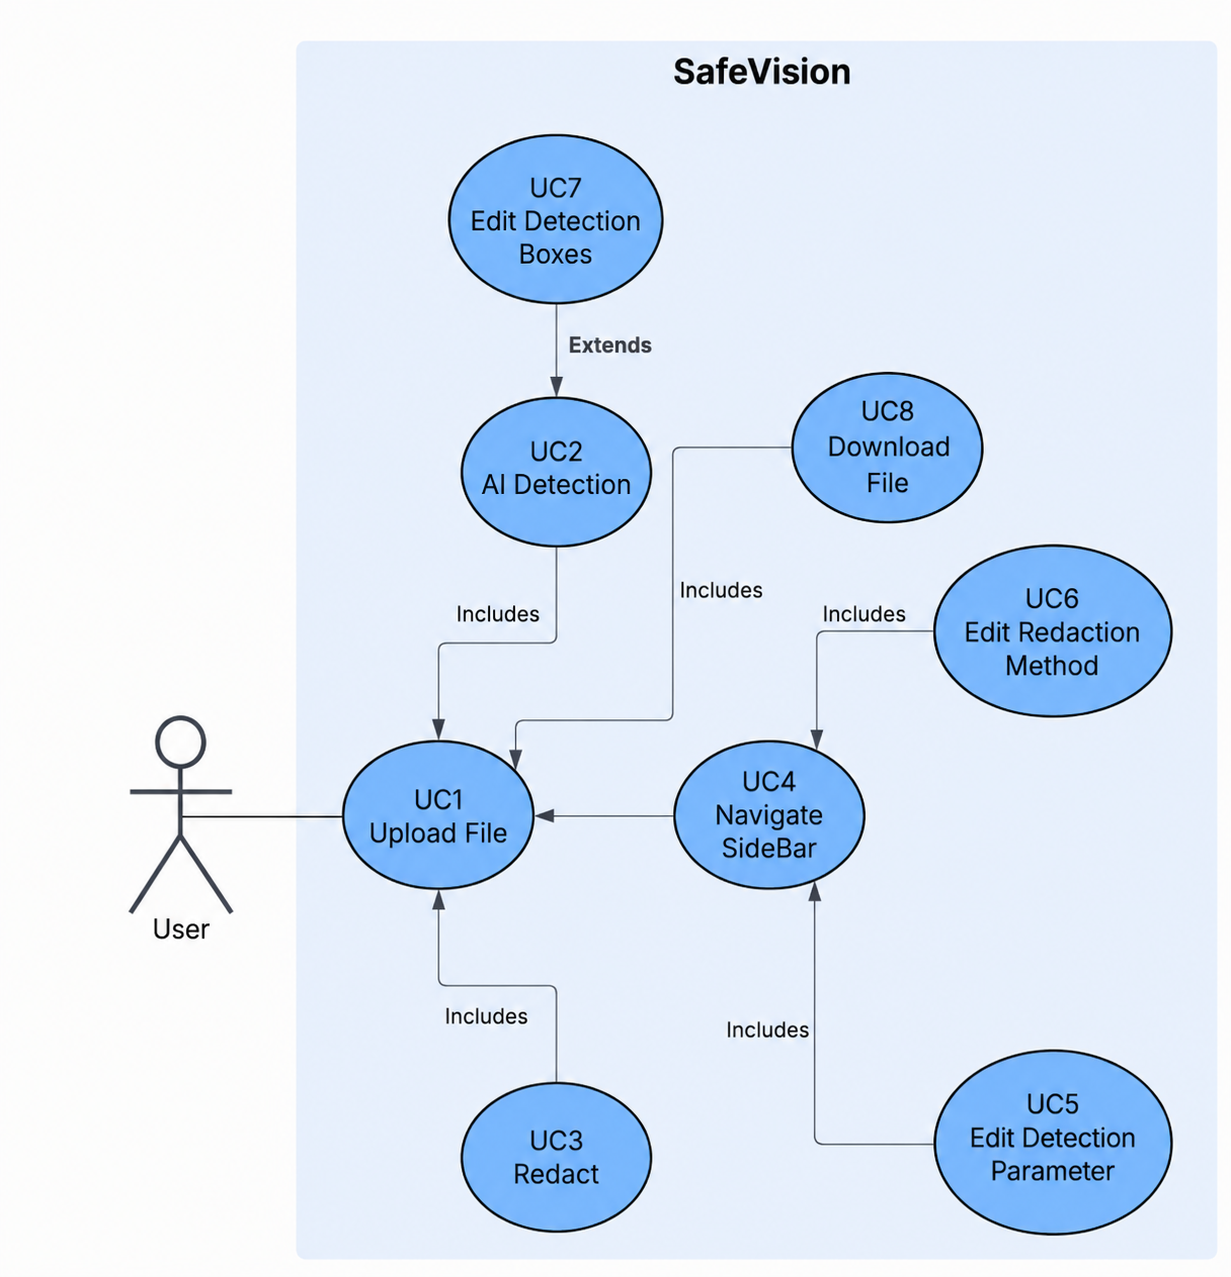
\includegraphics[width=0.8\textwidth]{figures/images/chapter-3/SafeVisionUseCase.png}
\caption{Use case diagram for the \gls{SafeVision} system}
\label{fig:safevision_usecase}
\end{figure}

\methodheading{Image Detection Scenario}

-As shown in Figure~\ref{fig:sequence_detection}, the image detection scenario begins when the user uploads an image through the interface and starts the detection process. \gls{SafeVision} then sends the image to the backend, where the relevant detection components analyze it and identify regions that may contain sensitive information. Once the analysis is complete, the detected regions are returned to the frontend and displayed as editable areas. Rather than being treated as final decisions, these results function as suggestions that the user can review, adjust, remove, or supplement with manually added regions before continuing. In this way, the workflow keeps the user in control of the detection outcome and reduces the risk of relying blindly on automated results.

\begin{figure}[H]
    \centering
    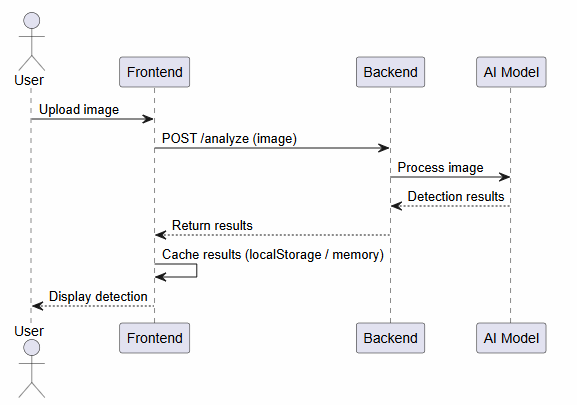
\includegraphics[width=0.9\textwidth]{figures/images/chapter-3/SequenceDetection.png}
    \caption{Sequence diagram illustrating the image detection interaction}
    \label{fig:sequence_detection}
\end{figure}

\methodheading{Redaction Scenario}

The redaction scenario follows the same overall interaction structure as the detection scenario shown in Figure~\ref{fig:sequence_detection}, but begins after the user has reviewed the detected regions. At this stage, the user decides which areas should be anonymized and selects an appropriate redaction method, such as blur, pixelation, or \gls{masking}. For standard redaction methods, the selected regions and settings are processed directly by the backend before the updated result is returned to the frontend. If the user instead selects \gls{segmentation} or \gls{inpainting}, the request is passed to the relevant AI-based processing components before the final result is generated. In both cases, the redacted output is presented to the user for verification before further use. This means that successful \gls{anonymization} depends not only on detecting relevant regions, but also on whether the final output sufficiently hides sensitive information.

Combined, these scenarios demonstrate how \gls{SafeVision} connects automated processing with user-guided verification. Detection and redaction are supported as linked workflow steps, while users can inspect and correct results before final \gls{anonymization}. As a result, the system supports both usability and reliability when handling sensitive information in visual media.

%------------------------- 4.3 ---------------------------

\section{Non-Functional Requirements}
\label{sec:nfr}

Beyond the core functional capabilities of detecting and redacting sensitive information, \gls{SafeVision} must satisfy several non-functional requirements that define the overall quality attributes of the system. These requirements guide architectural and implementation decisions by describing how the system should behave, rather than only what it should do. In this project, the non-functional requirements are categorized into four main areas: \textit{security}, \textit{performance}, \textit{usability}, and \textit{maintainability}, as illustrated in Figure~\ref{fig:non_functional_req}.

\begin{figure}[H]
    \centering
    \resizebox{0.92\textwidth}{!}{%
    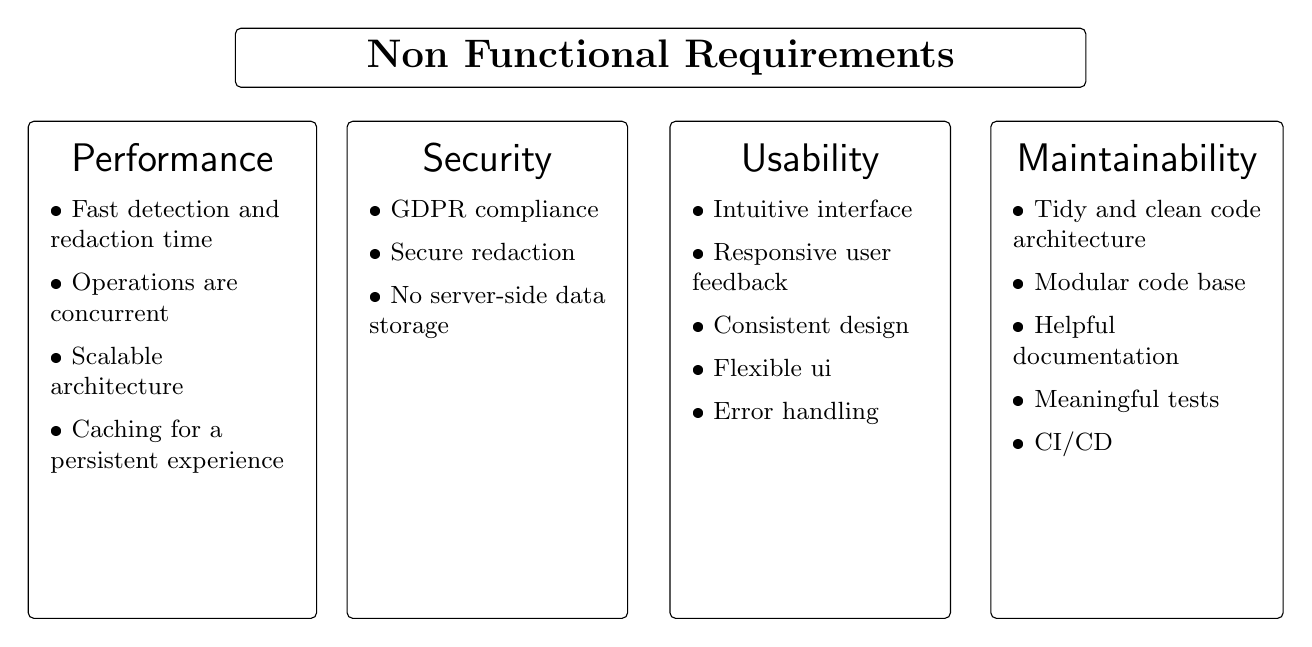
\begin{tikzpicture}[font=\sffamily]

        % Title
        \node[
            draw=black,
            fill=white,
            rounded corners=2pt,
            minimum width=10.8cm,
            minimum height=0.75cm,
            font=\bfseries\Large,
            align=center
        ] at (8.4,7.75) {Non Functional Requirements};

        % Performance
        \node[
            draw=black,
            fill=white,
            rounded corners=2pt,
            anchor=north,
            inner sep=8pt
        ] at (2.2,6.95) {%
            \parbox[t][5.75cm][t]{3.1cm}{%
                {\centering\Large Performance\par}
                \vspace{0.20cm}
                {\normalfont\small\raggedright
                \textbullet\ Fast detection and redaction time\par\vspace{0.16cm}
                \textbullet\ Operations are concurrent\par\vspace{0.16cm}
                \textbullet\ Scalable architecture\par\vspace{0.16cm}
                \textbullet\ Caching for a persistent experience\par}
            }%
        };

        % Security
        \node[
            draw=black,
            fill=white,
            rounded corners=2pt,
            anchor=north,
            inner sep=8pt
        ] at (6.2,6.95) {%
            \parbox[t][5.75cm][t]{3.0cm}{%
                {\centering\Large Security\par}
                \vspace{0.20cm}
                {\normalfont\small\raggedright
                \textbullet\ GDPR compliance\par\vspace{0.16cm}
                \textbullet\ Secure redaction\par\vspace{0.16cm}
                \textbullet\ No server-side data storage\par}
            }%
        };

        % Usability
        \node[
            draw=black,
            fill=white,
            rounded corners=2pt,
            anchor=north,
            inner sep=8pt
        ] at (10.3,6.95) {%
            \parbox[t][5.75cm][t]{3.0cm}{%
                {\centering\Large Usability\par}
                \vspace{0.20cm}
                {\normalfont\small\raggedright
                \textbullet\ Intuitive interface\par\vspace{0.16cm}
                \textbullet\ Responsive user feedback\par\vspace{0.16cm}
                \textbullet\ Consistent design\par\vspace{0.16cm}
                \textbullet\ Flexible \acrshort{ui}\par\vspace{0.16cm}
                \textbullet\ Error handling\par}
            }%
        };

        % Maintainability
        \node[
            draw=black,
            fill=white,
            rounded corners=2pt,
            anchor=north,
            inner sep=8pt
        ] at (14.45,6.95) {%
            \parbox[t][5.75cm][t]{3.15cm}{%
                {\centering\Large Maintainability\par}
                \vspace{0.20cm}
                {\normalfont\small\raggedright
                \textbullet\ Tidy and clean code architecture\par\vspace{0.16cm}
                \textbullet\ Modular code base\par\vspace{0.16cm}
                \textbullet\ Helpful documentation\par\vspace{0.16cm}
                \textbullet\ Meaningful tests\par\vspace{0.16cm}
                \textbullet\ CI/CD\par}
            }%
        };

    \end{tikzpicture}%
    }

    \caption{Overview of Non-Functional Requirements}
    \label{fig:non_functional_req}
\end{figure}

\subsubsection{Security}

Security requirements ensure that sensitive information is handled in a safe and responsible manner. Since the system processes images and videos that may contain personal data, the design should support GDPR-related principles such as data minimization, responsible processing, and reduced unnecessary storage. To support this, uploaded media should only be processed temporarily and should not be stored permanently on the server after the operation is complete. Secure redaction is therefore a central requirement, meaning that sensitive information should be anonymized before the processed output is used further. This reduces the risk of data breaches, unnecessary retention, and exposure of identifiable information while supporting the privacy oriented purpose of the system.

\subsubsection{Performance}

Performance requirements ensure that the system operates efficiently and provides a smooth user experience. Detection and redaction should be completed within a reasonable time so that users do not experience unnecessary delays when processing images or videos. This is especially important because \gls{SafeVision} includes \acrshort{ml} based analysis, which can be computationally demanding depending on the selected detection options, file size, and redaction method. The architecture should also support concurrent operations and be able to handle increasing workloads if the system is expanded further. Caching and client-side state handling can contribute to a more efficient user experience by reducing unnecessary repeated work and preserving relevant workflow information during interactions.

\subsubsection{Usability}

Usability requirements focus on making the system intuitive and understandable for users. Since \gls{SafeVision} is intended to support a workflow involving upload, detection, review, manual correction, redaction, and verification, the interface must make this sequence clear. Users should be able to understand what step they are in, what action is expected next, and whether the system is currently processing or waiting for input.

Responsive feedback is therefore important. Visual indicators, progress feedback, and clear messages help users understand the system state and the results of their actions. A consistent design across the application also makes navigation more predictable and reduces confusion. In addition, the interface should support flexibility by allowing users to adjust detection results, choose redaction methods, and correct errors before final output. Clear error handling is also necessary so that users can recover from issues without losing track of the workflow.

\subsubsection{Maintainability}

Maintainability requirements ensure that the system can be developed, updated, and extended over time. \gls{SafeVision} consists of several connected parts, including frontend interaction, backend services, \acrshort{ml} models, redaction logic, video processing, and deployment configuration. A modular codebase is therefore important because it separates responsibilities and makes it easier to modify one part of the system without affecting unrelated functionality.

Clean code structure, helpful documentation, and meaningful tests support long-term maintainability. Documentation makes the system easier to understand for new contributors, while tests help verify that important functionality continues to work when changes are introduced. CI/CD practices further support maintainability by enabling regular validation and deployment of updates. These requirements are important because the system should be designed in a way that allows for future improvement and extension.

%------------------------- 4.4 ---------------------------

\section{Requirement Prioritization}
\label{sec:priority}

To guide development and ensure that critical functionality was implemented first, the requirements were prioritized based on their importance, impact on the system, and input from Safe Media AI. The prioritization reflects a practical development approach, where essential functionality was implemented first, followed by desirable features, while less critical functionality was considered for potential future work.

\begin{itemize}
    \item \textbf{High Priority:}
    \begin{itemize}
        \item Automatic detection of sensitive information
        \item Manual editing capabilities
        \item Redaction functionality
        \item Image format support (PNG/JPEG)
    \end{itemize}

    \item \textbf{Medium Priority:}
    \begin{itemize}
        \item Multiple redaction methods
        \item Fast processing performance
        \item Video capabilities
    \end{itemize} 

    \item \textbf{Lower Priority:}
    \begin{itemize}
        \item Text Recognition capabilities
        \item Advanced customization options
        \item Inpaint redaction method
        \item Complex user preference options
        \item Metadata extraction and flexibility
    \end{itemize}
\end{itemize}

